%
% sphere.tex
%
% (c) 2021 Prof Dr Andreas Müller, OST Ostschweizer Fachhochschule
%
\documentclass[tikz]{standalone}
\usepackage{times}
\usepackage{amsmath}
\usepackage{txfonts}
\usepackage[utf8]{inputenc}
\usepackage{graphics}
\usetikzlibrary{arrows,intersections,math}
\usepackage{ifthen}
\begin{document}

\newboolean{showgrid}
\setboolean{showgrid}{false}
\def\breite{7}
\def\hoehe{4}

\begin{tikzpicture}[>=latex,thick]

\clip (-6.3,-2.95) rectangle (6.3,3.00);

% Povray Bild
\node at (-3.4,0) {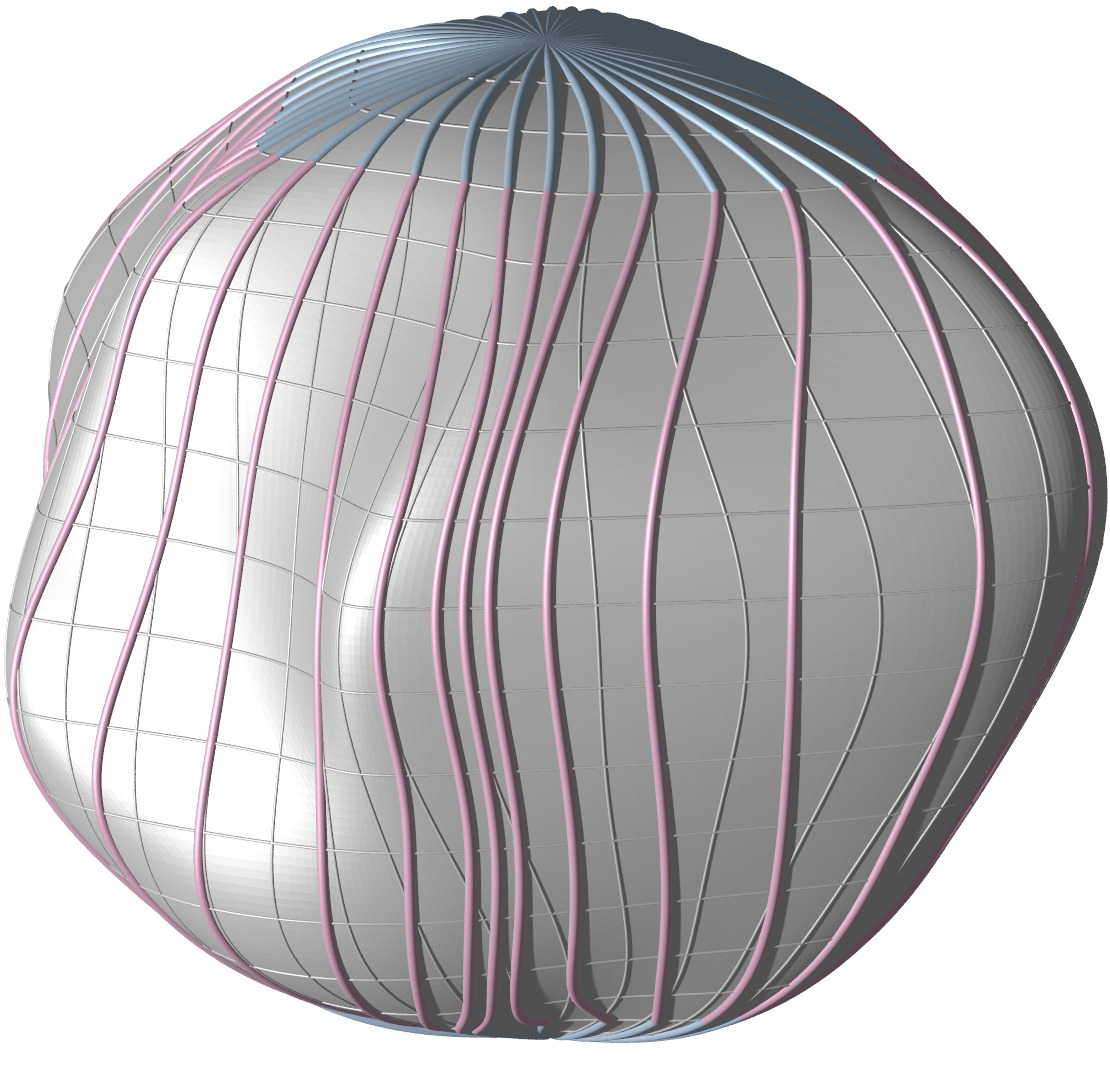
\includegraphics[height=5.5cm]{kartoffel.jpg}};
\node at (3.6,0) {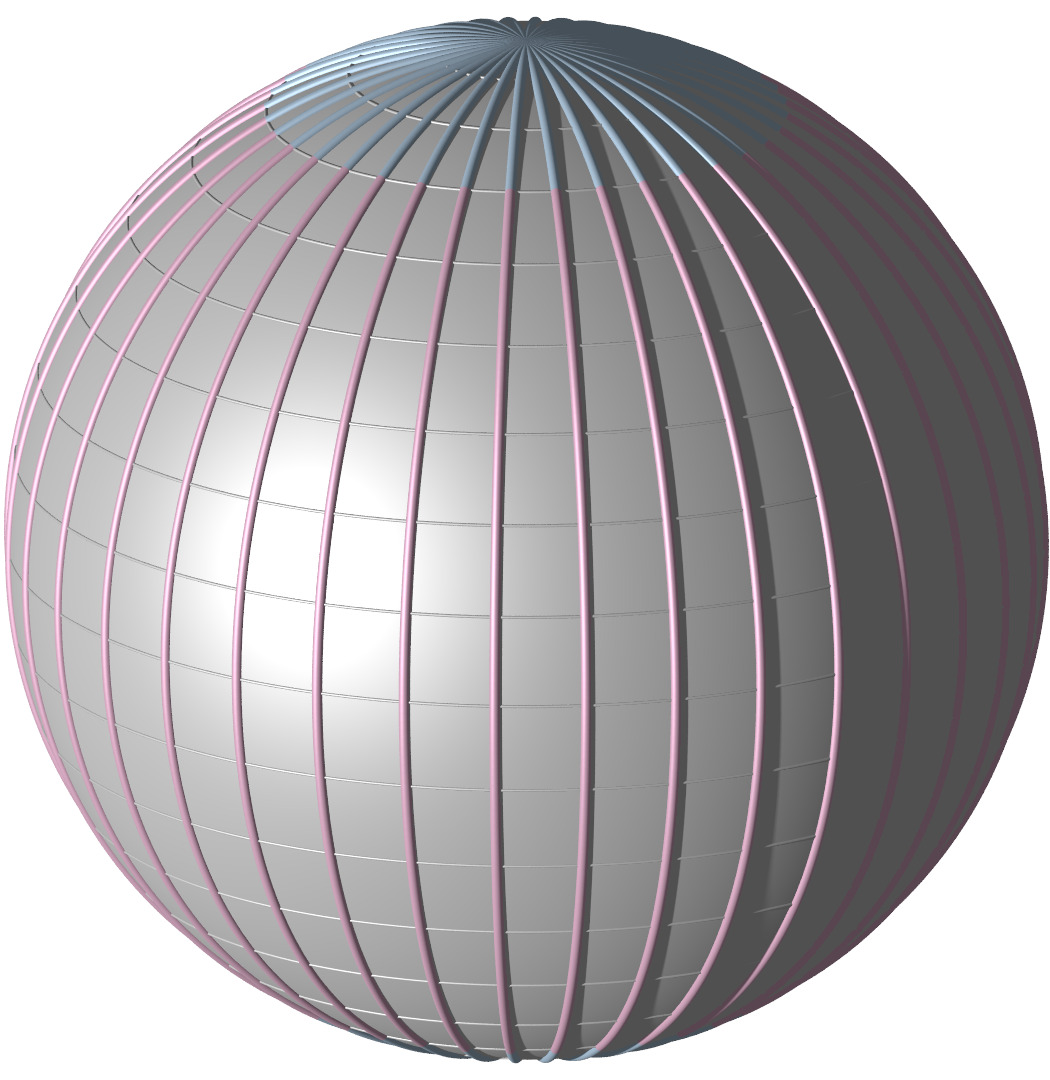
\includegraphics[height=5.5cm]{sphere.jpg}};

% Gitter
\ifthenelse{\boolean{showgrid}}{
\draw[step=0.1,line width=0.1pt] (-\breite,-\hoehe) grid (\breite, \hoehe);
\draw[step=0.5,line width=0.4pt] (-\breite,-\hoehe) grid (\breite, \hoehe);
\draw                            (-\breite,-\hoehe) grid (\breite, \hoehe);
\fill (0,0) circle[radius=0.05];
}{}

\node at (0.2,0) {$\longleftrightarrow$};

\begin{scope}[xshift=-3.4cm]
\node at (-2.75,2.25) [below right] {$M$};
\node at (0,2.85) {$N$};
\node at (0,-2.7) {$S$};
\end{scope}
\begin{scope}[xshift=3.6cm]
\node at (2.75,2.25) [below left] {$S^n$};
\node at (0,2.85) {$N$};
\node at (0,-2.8) {$S$};
\end{scope}

\end{tikzpicture}

\end{document}

